\chapter{Machine learning basics}

\section{Introduzione}
Il machine learning permette ai computer di acquisire conoscenza attraverso algoritmi che imparano e inferiscono dai dati.
Tale conoscenza viene rappresentata da un modello, che sulla base di esempi passati, imparerà a fare previsioni sui dati futuri.

	\subsection{Processo di learning}
	Si individua un processo di learning:
	\begin{multicols}{2}
		\begin{itemize}
			\item Acquisizione di dati dal mondo reale attraverso sensori.
			\item Preprocessamento dei dati: eliminazione del rumore, estrazione delle features e normalizzazione.
			\item Riduzione di dimensionalit\`a attraverso selezione e proiezione di features.
			\item Learning del modello: classification, regression, clustering e description.
			\item Test del modello attraverso cross-validation e bootstrap.
			\item Analisi dei risultati.
		\end{itemize}
	\end{multicols}

\section{Dati}
I dati disponibili ad un algoritmo di machine learning sono tipicamente un insieme di esempi.
Questi esempi sono tipicamente rappresentati come un array di features, caratteristiche dei dati di interesse per lo studio in atto, attraverso le feature il modello vede i dati.

	\subsection{Training, validation e test set}
	In particolare per questi algoritmi si assume sempre che il training, validation e il test set siano distribuiti secondo variabili indipendenti e identicamente distribuite (\emph{i.i.d}).
	La distribuzione $P_{data}$ \`e tipicamente sconosciuta ma si pu\`o campionare, attraverso un modello probabilistico di learning. Tipicamente il validation set \`e campionato dall'insieme di training.
	In particolare la distribuzione di probabilit\`a di coppie di esempio e label viene detta data generating distribution e sia il training data che il test set sono generati basandosi su di essa.
	
	Nota che non ci si può aspettare di ottenere buone performance da un modello di machine learning se i dati in ingresso non sono buoni. 
	Supponiamo di voler creare un modello che classifica foto di cani e gatti, i dati di training contengono 98 esempi di gatti e 2 cani. 
	Il modello imparerà a fornire la risposta che la foto contiene un gatto sbagliando solamente nel 2\% dei casi. 
	In fase di testing per\`o questo errore pu\`o essere molto pi\`u alto.
	\begin{figure}
		\centering
		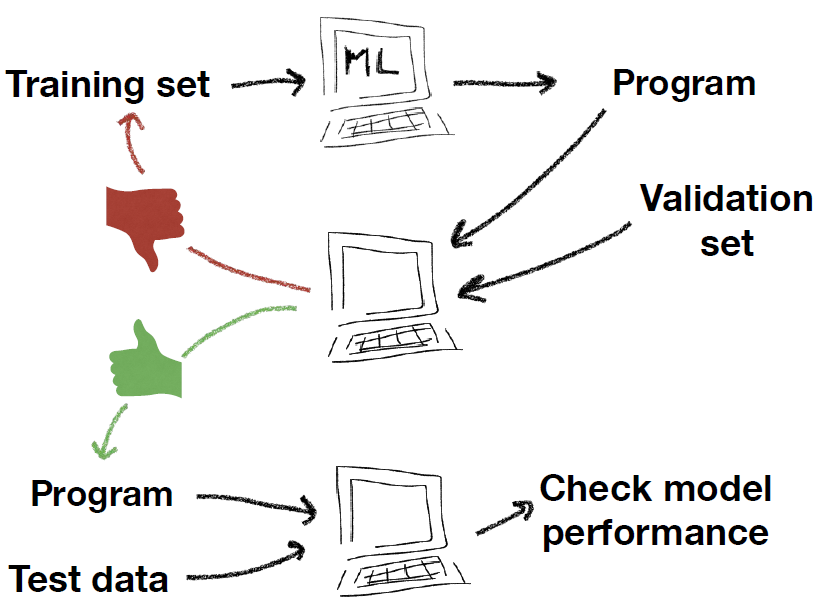
\includegraphics[width=0.4\linewidth]{imgs/chapter2/img0}
		\caption{Machine Learning Pipeline}
		\label{fig:chapter02-00}
	\end{figure}
\section{Task}
Si intende per task una rappresentazione del tipo di predizione che viene svolta per risolvere un problema su dei dati.
Viene identificata con un insieme di funzioni che possono potenzialmente risolverla.
In generale consiste di una funzione che assegna ogni input $x\in\mathcal{X}$ a un output $y\in\mathcal{Y}$:
$$f:\mathcal{X}\rightarrow\mathcal{Y}\qquad\mathcal{F}_{task}\subset\mathcal{Y^X}$$
La natura di $\mathcal{X},\mathcal{Y}, \mathcal{F}_{task}$ dipende dal tipo di task. 
Ad esempio, in un problema di classificazione Y è un insieme di etichette, in un problema di regressione è un numero reale.

\section{Modello}
Un modello \ref{fig:chapter02-01} \`e un programma per risolvere un problema.
\`E cio\`e l'implementazione di una funzione $f\in\mathcal{F}_{task}$ che pu\`o essere computata.
Un insieme di modelli formano uno spazio di ipotesi:
$$\mathcal{H}\subset\mathcal{F}_{task}$$
L'algoritmo cerca una soluzione nello spazio di ipotesi, altrimenti lo spazio sarebbe troppo grande.
Esistono diversi tipi di modello:
\begin{multicols}{2}
	\begin{itemize}
		\item Generativi e discriminativi.
		\item Parametrici e non parametrici.
	\end{itemize}
\end{multicols}

\begin{figure}
	\centering
	\begin{minipage}{.5\textwidth}
		\centering
		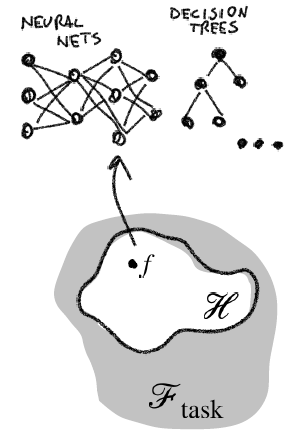
\includegraphics[width=0.4\linewidth]{imgs/chapter2/img1}
		\caption{Modello}
		\label{fig:chapter02-01}
	\end{minipage}%
	\begin{minipage}{.5\textwidth}
		\centering
		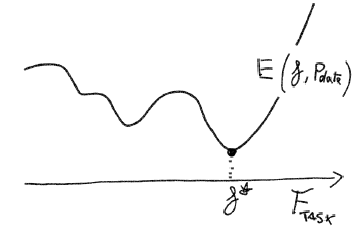
\includegraphics[width=1\linewidth]{imgs/chapter2/img2}
		\caption{Target ideale}
		\label{fig:chapter02-02}
	\end{minipage}
\end{figure}

	\subsection{Target ideale}
	Il target ideale \ref{fig:chapter02-02} del modello \`e quello di minimizzare una funzione di errore (generalizzazione)
	$$E(f;P_{data})$$
	Questa funzione determina quanto bene una soluzione $f\in\mathcal{F}_{task}$ approssima dei dati.
	Guida pertanto la selezione della migliore soluzione in $\mathcal{F}_{task}$.
	Pertanto:
	$$f^*\in arg\min\limits_{f\in\mathcal{F}_{task}}E(f;P_{data})$$
	
	\subsection{Target feasible}
	Si deve restringere il focus sul trovare funzioni che possono essere implementate e valutate in maniera trattabile. 
	Questa funzione potrebbe però non essere essere quella ottimale.
	Si definisce pertanto uno spazio di ipotesi del modello $\mathcal{H}\subset\mathcal{F}_{task}$ e si cerca la soluzione all'interno di quello spazio:
	$$f^*_{\mathcal{H}}\in arg\min\limits_{f\in\mathcal{H}} E(f;P_{data})$$
	Si noti come questa funzione non possa essere computata correttamente in quanto $P_{data}$ \`e sconosciuta. \ref{fig:chapter02-03}
	
	\subsection{Target attuale}
	Per trovare il target attuale \ref{fig:chapter02-04} si deve lavorare su un campione di dati o il training set
	$$\mathcal{D}_n=\{z_1,\dots,z_n\}$$
	Dove
	$$z_i=(x_i,y_i)\in\mathcal{X}\times\mathcal{Y}$$
	$$z_i\sim P_{data}$$
	Pertanto in:
	$$f^*_{\mathcal{H}}\in arg\min\limits_{f\in\mathcal{H}} E(f;D_{n})$$
	$E(f;D_{n})$ \`e il training error.
	\begin{figure}
		\centering
		\begin{minipage}{.5\textwidth}
			\centering
			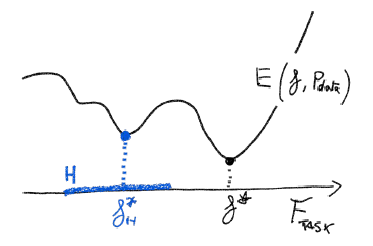
\includegraphics[width=1\linewidth]{imgs/chapter2/img3}
			\caption{Target feasible}
			\label{fig:chapter02-03}
		\end{minipage}%
		\begin{minipage}{.5\textwidth}
			\centering
			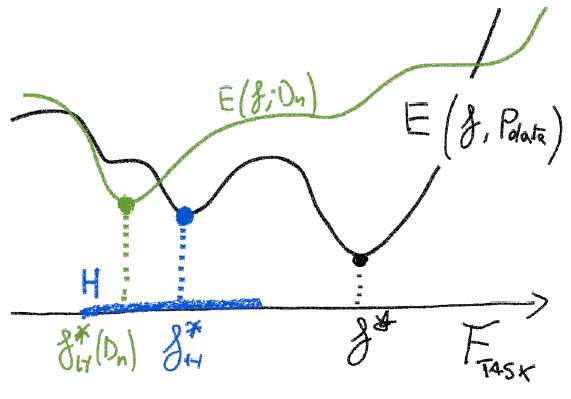
\includegraphics[width=1\linewidth]{imgs/chapter2/img4}
			\caption{Target attuale}
			\label{fig:chapter02-04}
		\end{minipage}
	\end{figure}
	
	\subsection{Funzione di errore}
	Le funzioni di generalizzazione e di training error possono essere scritte in termini di una pointwise loss $l(f;z)$ che misura l'errore che avviene a $f$ su un esempio di training $z$.
	$$E(f;P_{data})=\mathbb{E}_{z\sim P_{data}}[l(f;z)]$$
	$$E(f;\mathcal{D}_n)=\dfrac{1}{n}\sum\limits_{i=1}^nl(f;z_i)$$
	Si nota pertanto come l'algoritmo di learning \ref{fig:chapter02-05} risolve il problema di ottimizzazione con target:
	$$f^*_\mathcal{H}(\mathcal{D}_n)$$
	
	\subsection{Riassunto}
	Vorremmo operare sulla curva rossa \ref{fig:chapter02-06}, ma non possiamo farlo perch\`e non conosciamo $P_{data}$. 
	Possiamo operare solo sulla curva verde. 
	Successivamente dobbiamo restringere la ricerca allo spazio delle ipotesi $\mathcal{H}$ perch\`e $\mathcal{F}_{task}$ \`e troppo grande.
	Ci sono poi dei minimi locali che ci portano ad ottenere risultati molto elevati rispetto all'ottimo.
	
	
	\begin{figure}
		\centering
		\begin{minipage}{.5\textwidth}
			\centering
			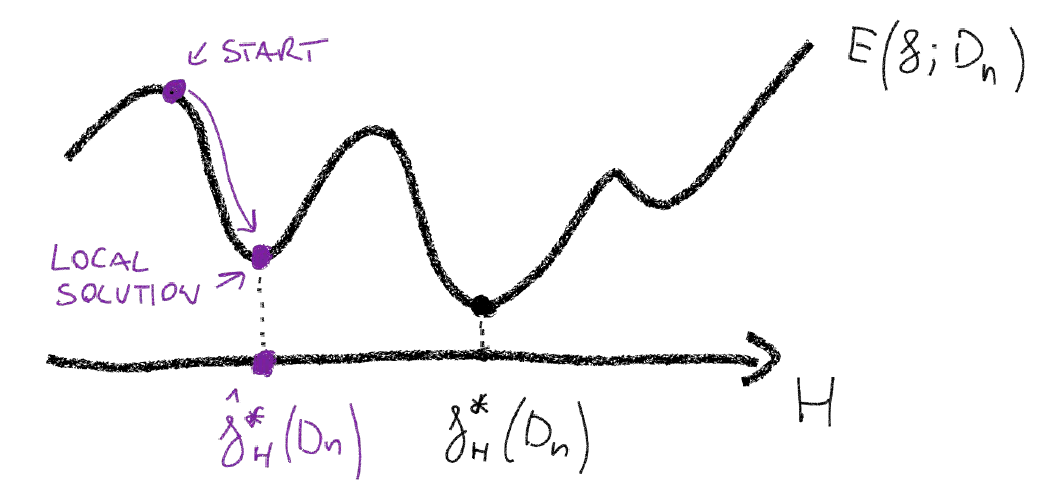
\includegraphics[width=1\linewidth]{imgs/chapter2/img5}
			\caption{Learning algorithm}
			\label{fig:chapter02-05}
		\end{minipage}%
		\begin{minipage}{.5\textwidth}
			\centering
			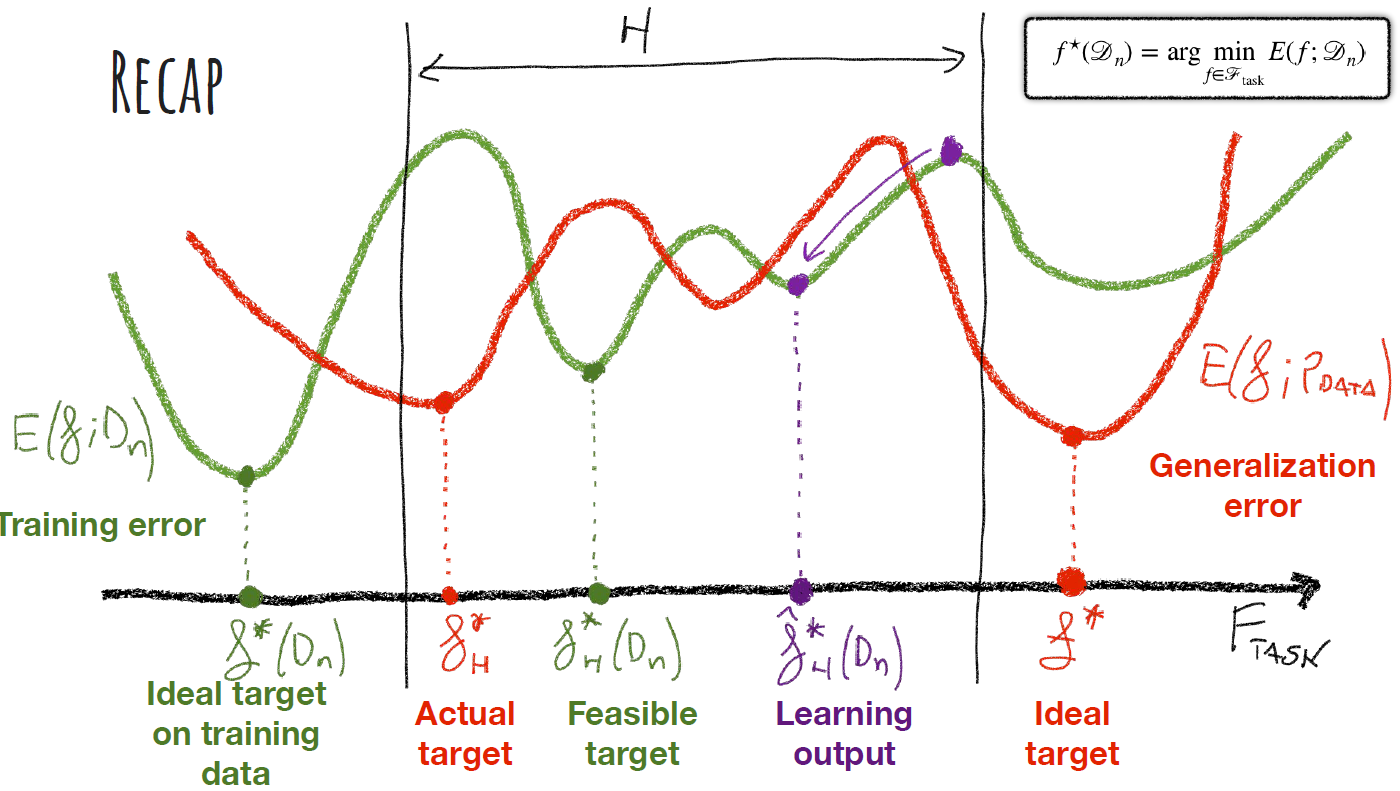
\includegraphics[width=1\linewidth]{imgs/chapter2/img6}
			\caption{Riassunto}
			\label{fig:chapter02-06}
		\end{minipage}
	\end{figure}
	
	\subsection{Tipi di errore}
	Rappresetazione grafica in \ref{fig:chapter02-11}.
	\begin{multicols}{2}
		\begin{itemize}
			\item Underfitting il modello non approssima sui dati di training, avviene per mancanza di dati, oppure perch\`e la fase di training \`e stata fermata troppo presto. Avremo scarse performance sul training e validation set.
			\item Overfitting quando i training data sono rumorosi e il modello li approssima perfettamente, ma impara un modello che si adatta solo su di essi e non approssima dati dal mondo reale. Ottime performance sul training e validation set, scarse sul test set.
			\item Estimation error, indotto imparando da un campione di dati.
			\item Approximation error, indotto dallo spazio di ipotesi $\mathcal{H}$, perché più piccolo di $\mathcal{F}_{task}$.
			\item Irreducible error a causa della variabilit\`a intrinseca. \`e un errore che non può essere rimosso anche scegliendo un modello diverso. Potrebbe essere causato da una scelta cattiva delle features.
		\end{itemize}
	\end{multicols}
	\begin{figure}
		\centering
		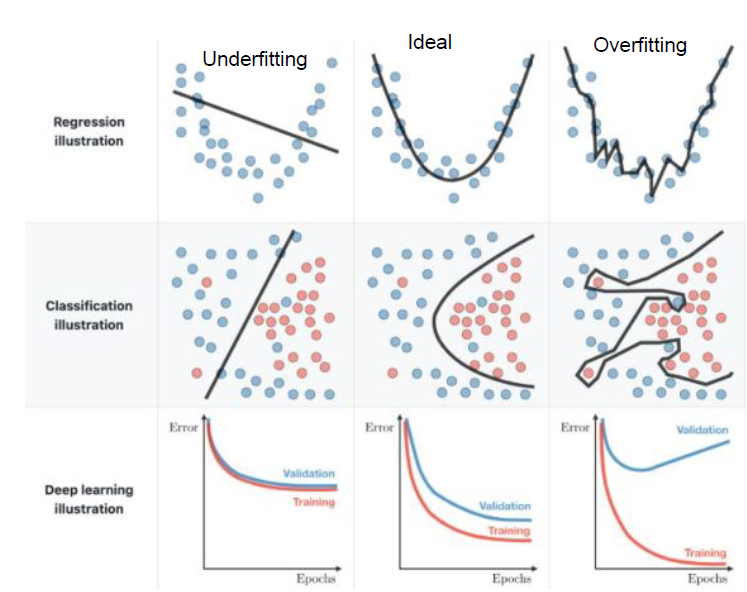
\includegraphics[width=0.6\linewidth]{imgs/chapter2/img11}
		\caption{Tipi di errore}
		\label{fig:chapter02-11}
	\end{figure}
	\subsection{Stimare l'errore di generalizzazione}
	L'errore di generalizzazione pu\`o essere stimato utilizzando diversi insiemi di training, validation e test.
	Si usa il training set per fare training di un modello, quello di validazione per valutarlo e sistemare i suoi iperparametri e dopo di quello si sceglie il modello migliore che si misura attraverso le performance sul test set.

	\subsubsection{Migliorare la generalizzazione}
	La generalizzazione pu\`o essere migliorata:
	\begin{multicols}{2}
		\begin{itemize}
			\item Evitando di ottenere il minimo sul training error. 
			\item Riducendo la capacit\`a del modello.
			\item Cambiando l'obiettivo con un termine di regolarizzazione.
			\item Iniettando rumore nell'algoritmo. 
			\item Fermando l'algoritmo prima che converga. Noto come early stopping, quindi si termina prematuramente la fase di training.
			\item Aumentantdo la quantit\`a di dati.
			\item Aggiungendo pi\`u campioni di training. In un modello che etichetta le immagini possiamo pensare di applicare trasformazioni alle immagini ruotandole, traslandole.
			\item Aumentando il training set con trasformazioni.
			\item Combinando predizioni da pi\`u modelli decorrelati o ensembling.
		\end{itemize}
	\end{multicols}
	
	\paragraph{Regolarizzazione}
	Si intende per regolarizzazione \ref{fig:chapter02-07} la modifica della funzione di training error con un termine $\Omega(f)$ che penalizza soluzioni complesse:
	$$E_{reg}(f;\mathcal{D}_n)=E(f;\mathcal{D}_n)+\lambda_n\Omega(f)$$
	In questa equazione $\lambda$ \`e un iperparametro.
	
	\begin{figure}
		\centering
		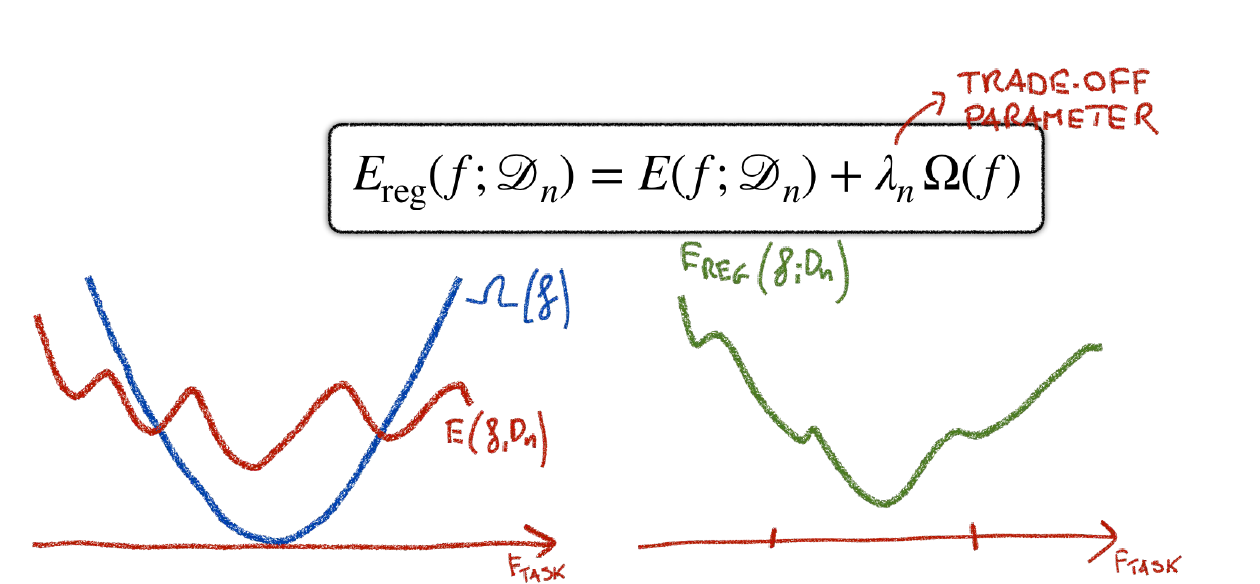
\includegraphics[width=0.6\linewidth]{imgs/chapter2/img7}
		\caption{Regolarizzazione}
		\label{fig:chapter02-07}
	\end{figure}

\section{Tipi di learning}

	\subsection{Supervised learning}
	Nel supervised learning vengono dati in input a un modello o predittore un insieme di esempi che possiedono una label.
	Il modello poi impara a creare delle predizioni su un nuovo esempio.

		\subsubsection{Dati}
		Nel caso del supervised learning i dati creano una distribuzione:
		$$p_{data}\in\Delta(\mathcal{X}\times\mathcal{Y})$$
		
		\subsubsection{Classificazione}
		In un problema di classificazione si trova un insieme finito di label discrete.
		In particolare dato un training set $\mathcal{T} = \{(x_1, y_1),\dots(x_m, y_m)\}$, si deve imparare una funzione $f$ per predirre $y$ dato $x$.
		$f$ sar\`a pertanto:
		$$f:\mathbb{R}^d \rightarrow\{1, 2, \dots, k\}$$
		Dove $d$ \`e la dimensionalit\`a di $x$ e $k$ il numero di labels distinte.
		
		\paragraph{Task}
		Si deve pertanto trovare una funzione $f\in\mathcal{Y^X}$ che assegna ogni input $x\in\mathcal{X}$ a una label discreta.
		$$f(x)\in\mathcal{Y}=\{c_1,\dots,c_k\}$$
		\paragraph{Applicazioni}
		\begin{multicols}{2}
			\begin{itemize}
				\item Riconoscimento dei volti.
				\item Riconoscimento dei caratteri.
				\item Rilevamento dello spam.
				\item Diagnosi medica: dai sintomi alle malattie.
			\end{itemize}
		\end{multicols}
		
		\subsubsection{Regression}
		Un problema di regressione presenta un insieme di label continue.
		Dato un training set $\mathcal{T}=\{(x_1, y_1),\dots,(x_m,y_m)\}$, si deve imparare una funzione $f$ per predirre $y$ dato $x$.
		$f$ sar\`a pertanto:
		$$f:\mathbb{R}^d\rightarrow\mathbb{R}$$
		Dove $d$ \`e la dimensionalit\`a di $x$.
		
		\paragraph{Task}
		Si deve trovare una funzione $f(x)\in\mathcal{Y}$ che assegna ogni input a una label continua.
		\paragraph{Applicazioni}
		\begin{multicols}{2}
			\begin{itemize}
				\item Economia/Finanza: prevedere il valore di un titolo azionario.
				\item Epidemiologia.
				\item Navigazione in auto/aereo: angolo del volante, accelerazione.
				\item Tendenze temporali: tempo atmosferico nel tempo.
			\end{itemize}
		\end{multicols}
		\subsubsection{Ranking}
		Il ranking \`e un tipo particolare di classificazione in cui una label \`e un ranking.
		
		\paragraph{Applicazioni}
		\begin{multicols}{2}
			\begin{itemize}
				\item Data una query e un insieme di pagine web, classificarle in base alla rilevanza..
				\item Data un'immagine, trovare le immagini visivamente più simili nel database.
				\item Preferenze dell'utente, ad esempio "La mia lista" di Netflix 
			\end{itemize}
		\end{multicols}
		
	\subsection{Unsupervised learning}
	Nell'unsupervised learning vengono dati in input a un modello o predittore un insieme di esempi senza label.
	Il modello impara a creare delle predizioni su un nuovo esempio.
		
		\subsubsection{Dati}
		Nel caso dell'unsupervised learning i dati creano una distribuzione:
		$$p_{data}\in\Delta(\mathcal{X})$$
		\subsubsection{Denisty estimation}
		Nel density estimation si cerca una distribuzione di probabilità $f\in\Delta(\mathcal{X})$ che fitta $x\in\mathcal{X}$.
		
		\paragraph{Task}
		Stiamo facendo una stima dei parametri della gaussiana sottostante ai dati.
		
		\paragraph{Applicazioni}
		\begin{multicols}{2}
			\begin{itemize}
				\item Può essere utilizzato per rilevare anomalie, se un punto si allontana dalla "media".
				\item Può essere utilizzato anche per generare nuovi dati perché si conosce la distribuzione.
			\end{itemize}
		\end{multicols}
		
		\subsubsection{Clustering}
		Nel clustering, data $\mathcal{T}=\{x_1, \dots, x_m\}$ si deve trovare la struttura nascosta che intercorre tra le $x$ o i clusters.
		
		\paragraph{Task}
		Si deve trovare una funzione $f\in\mathbb{N}^{\mathcal{X}}$ che assegna ogni input $x\in\mathcal{X}$ a un indice di cluster $f(x)\in\mathbb{N}$.
		Tutti i punti mappati sullo stesso indice formano un cluster.
		
		\paragraph{Applicazioni}
		\begin{multicols}{2}
			\begin{itemize}
				\item Analisi delle reti sociali.
				\item Genomica: raggruppare gli individui in base alla somiglianza genetica.
				\item Rilevamento di anomalie: Analizzare un insieme di eventi o oggetti e individuare alcuni di essi come insoliti o atipici, ad esempio: rilevamento di frodi con carte di credito, sorveglianza video.
				\item Segmentazione delle immagini.
			\end{itemize}
		\end{multicols}

	\subsubsection{Dimensionality reduction}
	Nella dimensionality reduction si tenta di ridurre il numero di variabili sotto considerazione ottenendo un insieme di variabili principali.

		\paragraph{Task}
		Si deve trovare una funzione $f\in\mathcal{Y}^\mathcal{X}$ che mappa ogni input di molte dimensioni $x\in\mathcal{X}$ a un output a dimensione minore $f(x)\in\mathcal{Y}$, dove $dim(\mathcal{Y})\ll dim(\mathcal{X})$

	\subsection{Reinforcement learning}
	Nel reinforcement learning un agente impara dall'ambiente interagendo con esso e ricevendo premi per lo svolgimento di azioni particolari.
	In particolare, data una sequenza di esempi o stati e una reward dopo il completamento di tale sequenza si impara a predirre l'azione da svolgere per uno stato o esempio individuale.

\section{Polynomial curve fitting}

	\subsection{Dati}
	L'insieme dei dati $\mathcal{D}_n$ consiste di coppie:
	$$\mathcal{D}_n = \{(x_1, y_1),\dots,(x_n,y_n)\}$$
	I dati sono generati dalla funzione $\sin(2\pi x)$ con del rumore.
	Il training set consiste di $10$ punti: $n = 10$. \ref{fig:chapter02-09}

	\subsection{Modello e spazio di ipotesi}
	Il modello per il Polynomial curve fitting \ref{fig:chapter02-10} \`e:
	$$f_w(x) = \sum\limits_{j = 0}^M w_jx^j$$
	\`E parametrico, dove i parametri sono $\{w_0,\dots, w_m\}$.
	Lo spazio di ipotesi per $M\in\mathbb{N}$ fissato \`e:
	$$\mathcal{H}_M = \{f_w:w\in\mathbb{R}^M\}$$


	\begin{figure}
		\centering
		\begin{minipage}{.5\textwidth}
			\centering
			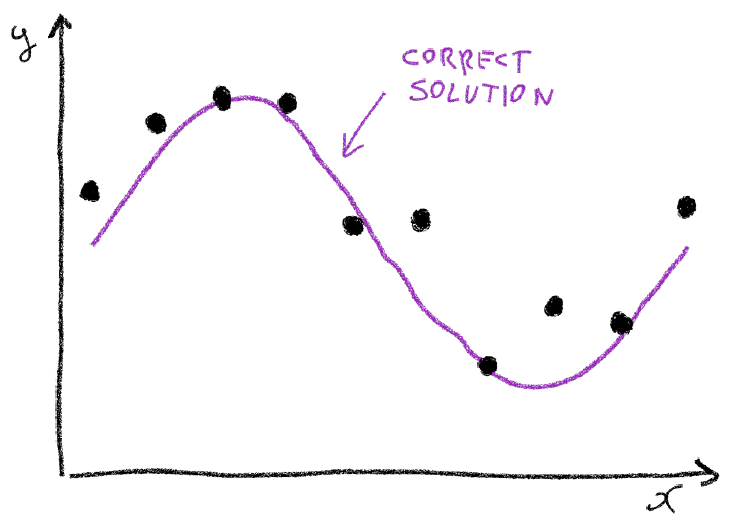
\includegraphics[width=1\linewidth]{imgs/chapter2/img9}
			\caption{Polynomial curve fitting}
			\label{fig:chapter02-09}
		\end{minipage}%
		\begin{minipage}{.5\textwidth}
			\centering
			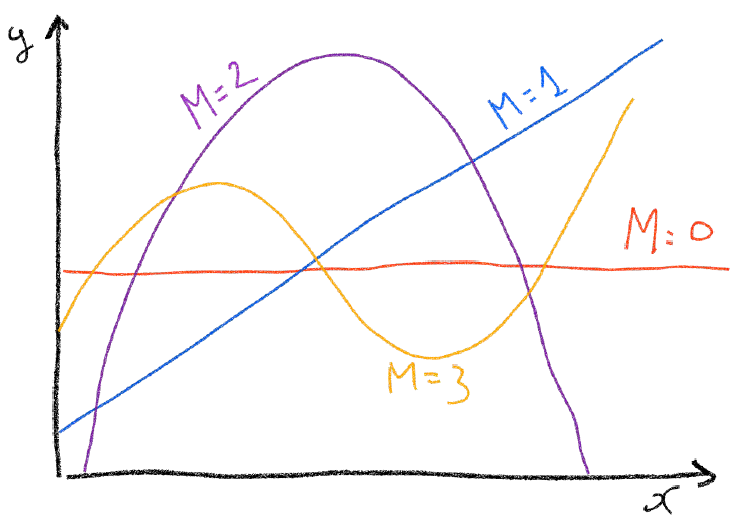
\includegraphics[width=1\linewidth]{imgs/chapter2/img10}
			\caption{Polynomial curve fitting}
			\label{fig:chapter02-10}
		\end{minipage}
	\end{figure}



	\subsection{Error function}
	La funzione di errore per il polynomial curve fitting consiste della media tra le distanze quadratiche tra la predizione effettuata e l'effettiva label.
	La pointwise loss:
	$$l(f;(x_i,y_i)) = [f(x_i) - y_i]^2$$
	La funzione di errore \`e pertanto:
	$$E(f;\mathcal{D}_n) = \mathbb{E}(l(f;(x_i,y_i))) = \frac{1}{n}\sum\limits_{i=1}^n[f(x_i)-y_i]^2$$

	\subsection{Funzione obiettivo}
	Si ricordi che la funzione obiettivo \`e:
	$$f^*_{\mathcal{H}_M}(\mathcal{D}_n)\in\arg\min\limits_{f\in\mathcal{H}_M}E(f;\mathcal{D}_n)$$
	Equivalente rispetto a $f_{w^*}$ dove:
	$$w^*\in\arg\min\limits_{w\in\mathbb{R}^M}\frac{1}{n}\sum\limits_{i=1}^n[f_w(x_i)-y_i]^2$$
	A parole: trovare i pesi che minimizzano l'errore. 
	Si noti come questa richieda la risoluzione di un sistema lineare di equazioni.
	Il cambiamento di $M$ influisce grandemente sull'accuratezza della predizione, andando a determinare casi di overfitting o underfitting \ref{fig:chapter02-12}.
	Con questo caso particolare si trova la soluzione migliore con $M=3$.
	
	\begin{figure}
		\centering
		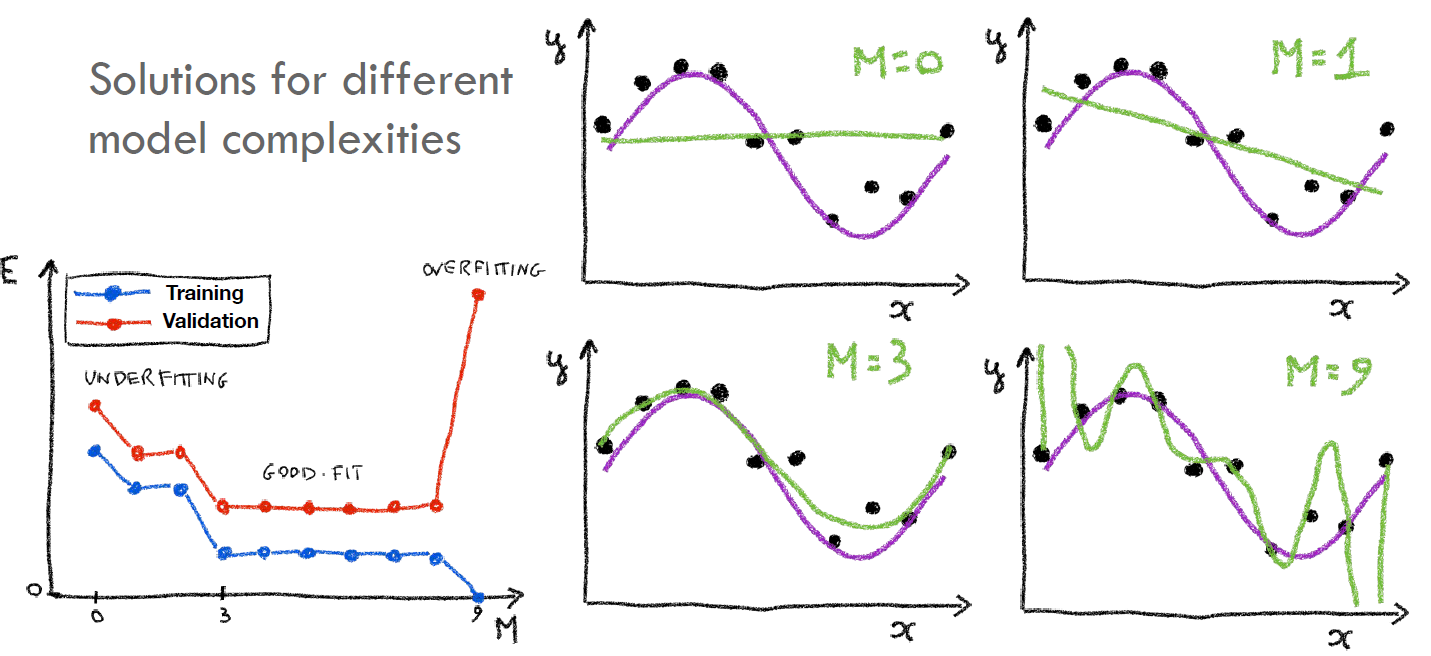
\includegraphics[width=0.6\linewidth]{imgs/chapter2/img12}
		\caption{Overfitting e underfitting nel Polynomial curve fitting}
		\label{fig:chapter02-12}
	\end{figure}
	
	\subsection{Regolarizzazione}
	Il polynomial curve fitting \ref{fig:chapter02-8} si regolarizza penalizzando i polinomi con grandi coefficienti:
	$$E_{reg}(f_w;\mathcal{D}_n) = \frac{1}{n}\sum\limits_{i=1}^n[f_w(x_i)-y_i]^2 + \frac{\lambda}{n}||w||^2$$
	Dove $||w||^2 = \sum\limits_{i = 1}^n w_i^2$.
	
	\begin{figure}
		\centering
		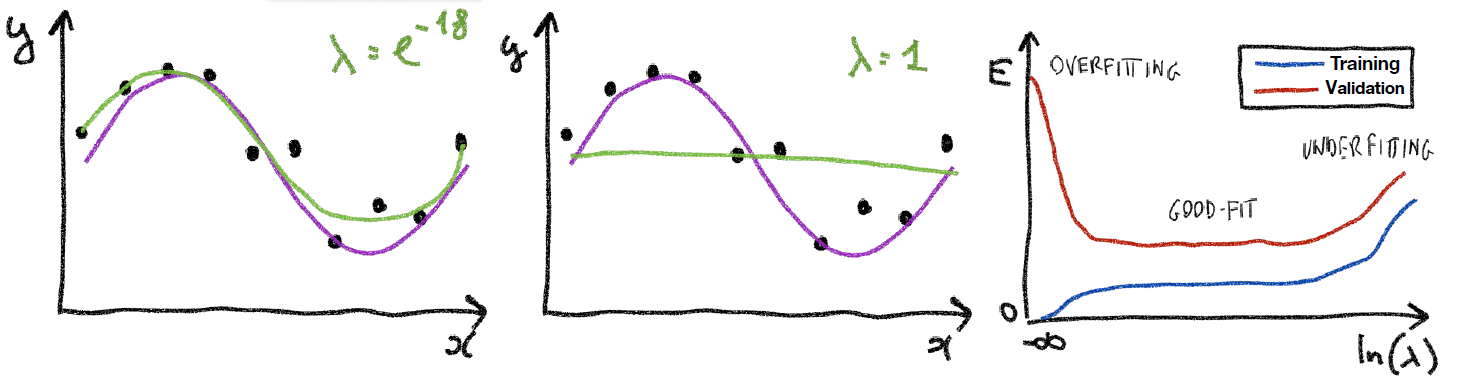
\includegraphics[width=0.6\linewidth]{imgs/chapter2/img8}
		\caption{Regolarizzazione nel Polynomial Curve Fitting}
		\label{fig:chapter02-8}
	\end{figure}
